\documentclass[utf8]{beamer}
\usepackage[utf8]{inputenc}
\usepackage[T1]{fontenc}
\usepackage[brazilian]{babel}
\usepackage{listings}
\usepackage{xcolor}

\lstset{
	language=Python,
	basicstyle=\ttfamily\small,
	commentstyle=\color{gray},
	keywordstyle=\color{blue},
	stringstyle=\color{red},
	showstringspaces=false,
	breaklines=true,
	frame=single
}
\usepackage{amsmath}
\usepackage{amssymb}
\usepackage[utf8]{inputenc}
\usepackage[T1]{fontenc}
\usepackage{beamerthemesplit}
\usepackage[orientation=landscape,size=custom,width=16,height=9,scale=0.5,debug]{beamerposter} 
\usepackage{amsmath, amsthm, amssymb}
\usepackage{mathtools}
\usepackage[utf8]{inputenc}
\usepackage[T1]{fontenc}
\usefonttheme[onlymath]{serif}
\usepackage{hyperref}
%\usepackage{times} 
\usepackage{lmodern}
\usepackage{verbatim}
\usepackage{listings}
\lstset{language=python, basicstyle=\ttfamily\footnotesize}
%\usetheme{Antibes}
\usepackage{subfigure, graphics, graphicx}
\usetheme{Copenhagen}
\defbeamertemplate*{footline}{mysplit theme}
  {%
	\leavevmode%
	\hbox{\begin{beamercolorbox}[wd=.5\paperwidth,ht=2.5ex,dp=1.125ex,leftskip=.3cm plus1fill,rightskip=.3cm]{author in head/foot}%
			\usebeamerfont{author in head/foot}\insertshortauthor
		\end{beamercolorbox}%
		\begin{beamercolorbox}[wd=.5\paperwidth,ht=2.5ex,dp=1.125ex,leftskip=.3cm,rightskip=.3cm plus1fil]{title in head/foot}%
			\usebeamerfont{title in head/foot}\insertshorttitle\hfill
			\insertframenumber/\inserttotalframenumber\hspace*{0.5em}
	\end{beamercolorbox}}%
	\vskip0pt%
}




\theoremstyle{definition}
\newtheorem{teo}{Teorema}
\newtheorem{mydef}{Definição}
\newcommand{\R}{\mathbb{R}}


\begin{document}
	\author{ Bruno Dalcantoni Cozac \\
		  	 Gabriel de Oliveira Bispo\\
			 Deyvisson Nascimento Garcês \\
			 Victor Matheus da Cunha Santos \\ }
	\title{Assingmnent 01 - Cache miss na multiplicação de matrizes}
	\subtitle{Introdução à computação paralela e medidas de performance}
	\logo{figures/logoppgmmc}
	\institute{ICMC-USP \\ \noindent Disciplina: SME5873/SME0252 \\
	Professor: Prof. Fabrício Simeoni de Sousa  \& \\
	Luan da Fonseca Santos }
	%\date{}
	\subject{}
	\setbeamercovered{transparent}
	\setbeamertemplate{navigation symbols}{}

	\begin{frame}[plain]
		\maketitle
	\end{frame}




\begin{frame}
		\frametitle{Performance em MATLAB}
	\begin{figure}[H]
		\centering
		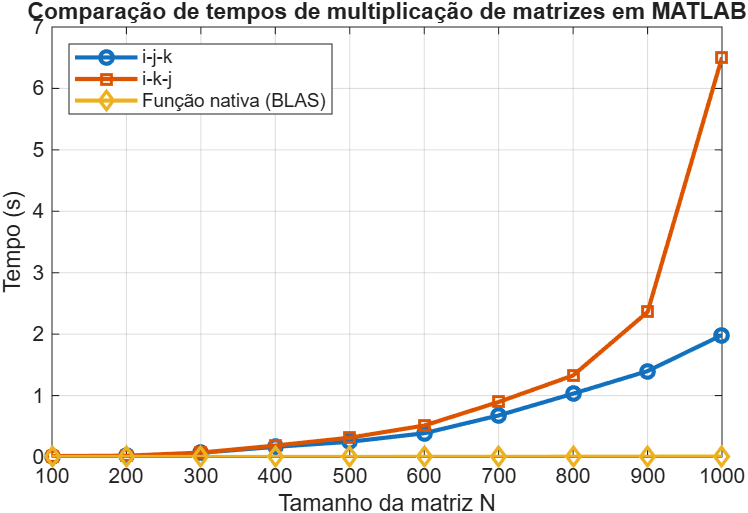
\includegraphics[width=0.5\linewidth]{../matlab/untitled1.png}
		\caption{MATLAB}
		\label{fig:matmultr2022}
	\end{figure}
	
\end{frame}
\begin{frame}
	\begin{itemize}
		\item Compilador interno \textit{Just-In-Time (JIT)}
	\end{itemize}
\end{frame}


\begin{frame}
	\frametitle{Performance em C}
	\begin{figure}[H]
		\centering
		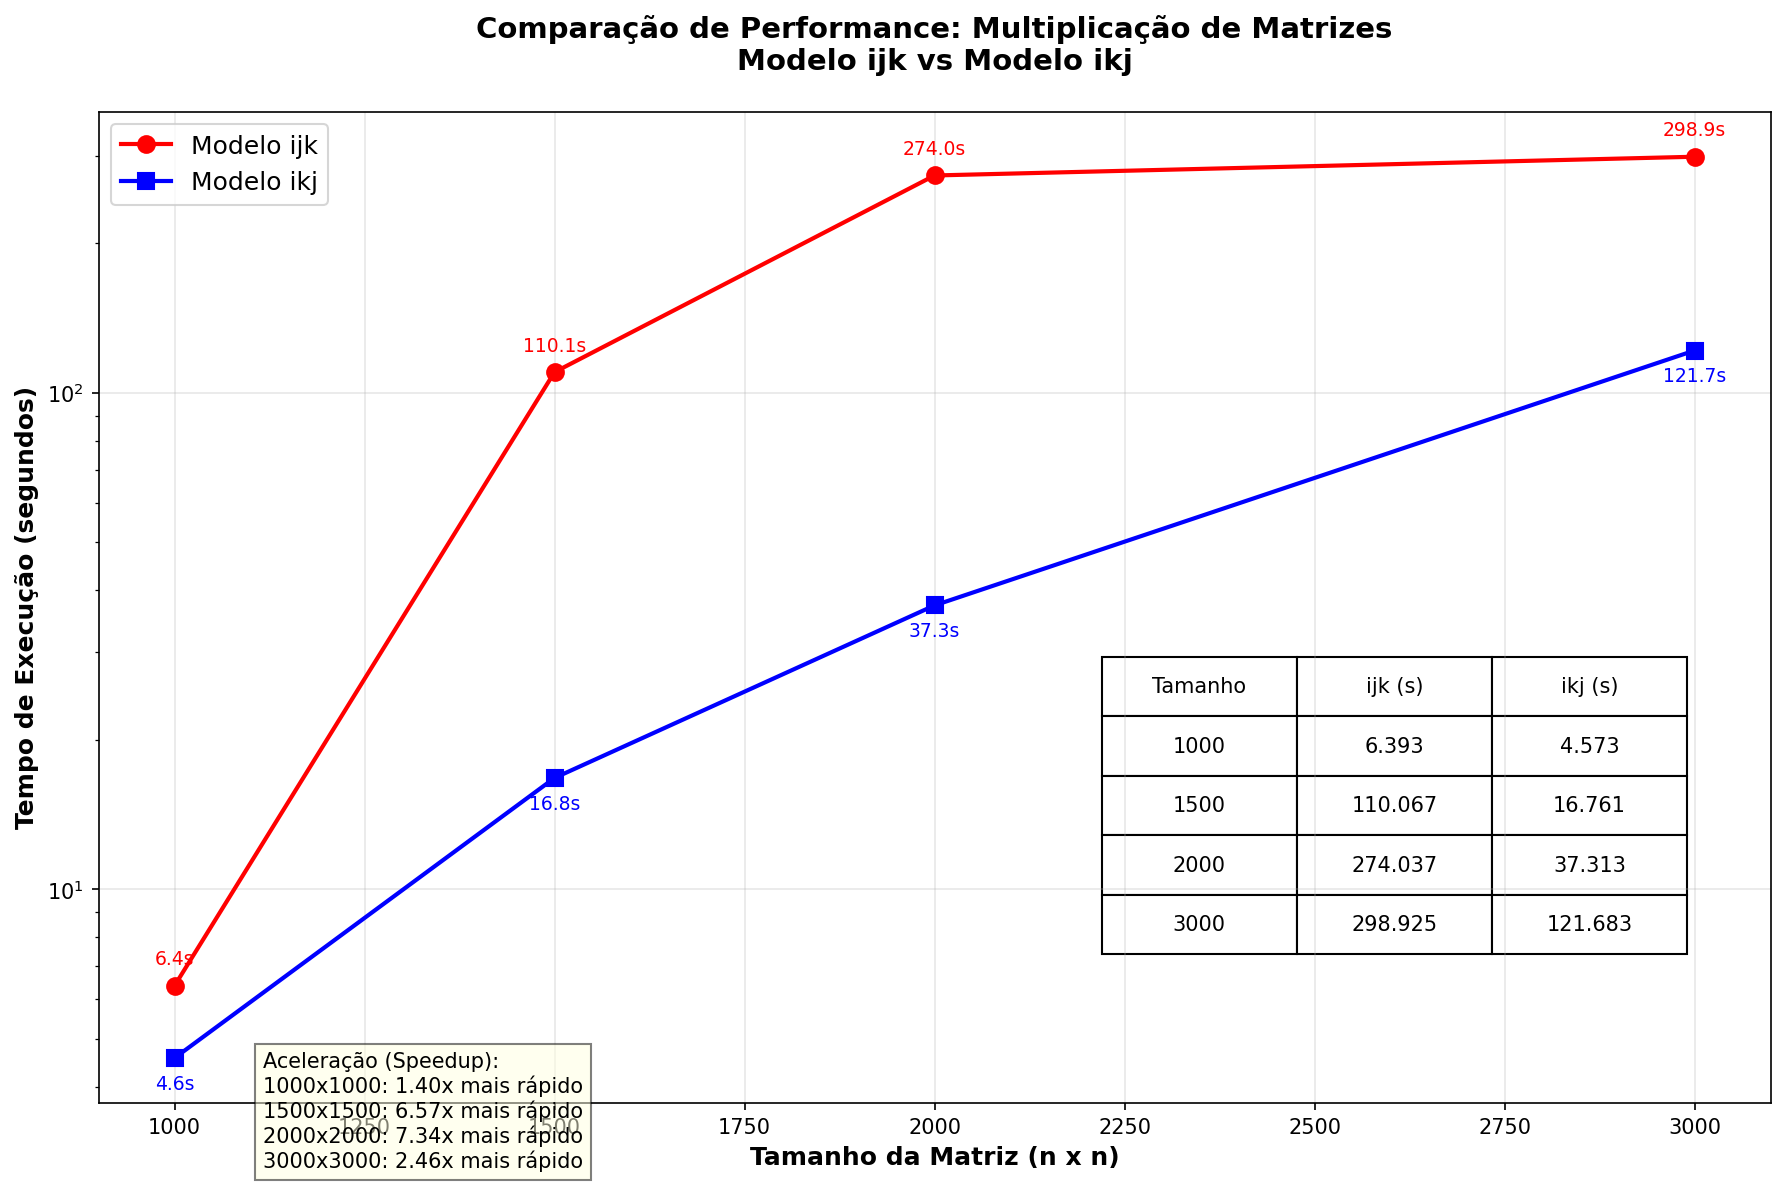
\includegraphics[width=0.65\linewidth]{Figuras/performance_multiplicacao_matrizes}
		\caption{C}
		\label{fig:performace_c}
	\end{figure}
	
\end{frame}

\begin{frame}[fragile]
	\frametitle{Parâmetros}
	\begin{itemize}
		\item Usamos um intervalo de -10000 a 1000 para os valores nas matrizes
	\end{itemize}
	\begin{lstlisting}
		row[j] = random.randint(-10000, 10000)
	\end{lstlisting}

\end{frame}

\begin{frame}[fragile]
	\frametitle{Ordem de Loop}
	\begin{semiverbatim}
		# Ordem ijk (mais lenta)
		for i in range(n):
		   for j in range(n):
		      for k in range(n):  # Acesso não-sequencial à memória
		        C[i][j] += A[i][k] * B[k][j]
		
		# Ordem ikj (mais rápida)
		for i in range(n):
		   for k in range(n):
		      for j in range(n):  # Acesso sequencial à memória
		         C[i][j] += A[i][k] * B[k][j]
	\end{semiverbatim}
\end{frame}

\begin{frame}
	\frametitle{Performance em Python}
	\begin{figure}[H]
		\centering
		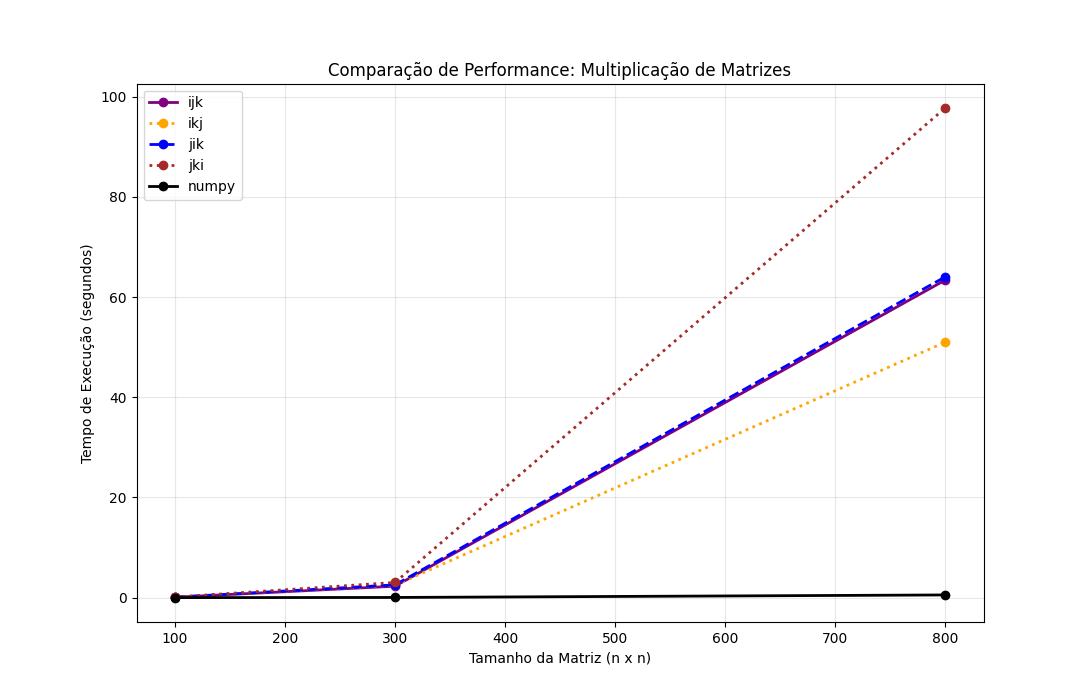
\includegraphics[width=0.80\linewidth]{Figuras/cachemiss_python}
		\caption{Python}
		\label{fig:performace_python}
	\end{figure}
\end{frame}

\begin{frame}
		\frametitle{Pyhton vs Matlab}
	\begin{figure}[H]
		\centering
		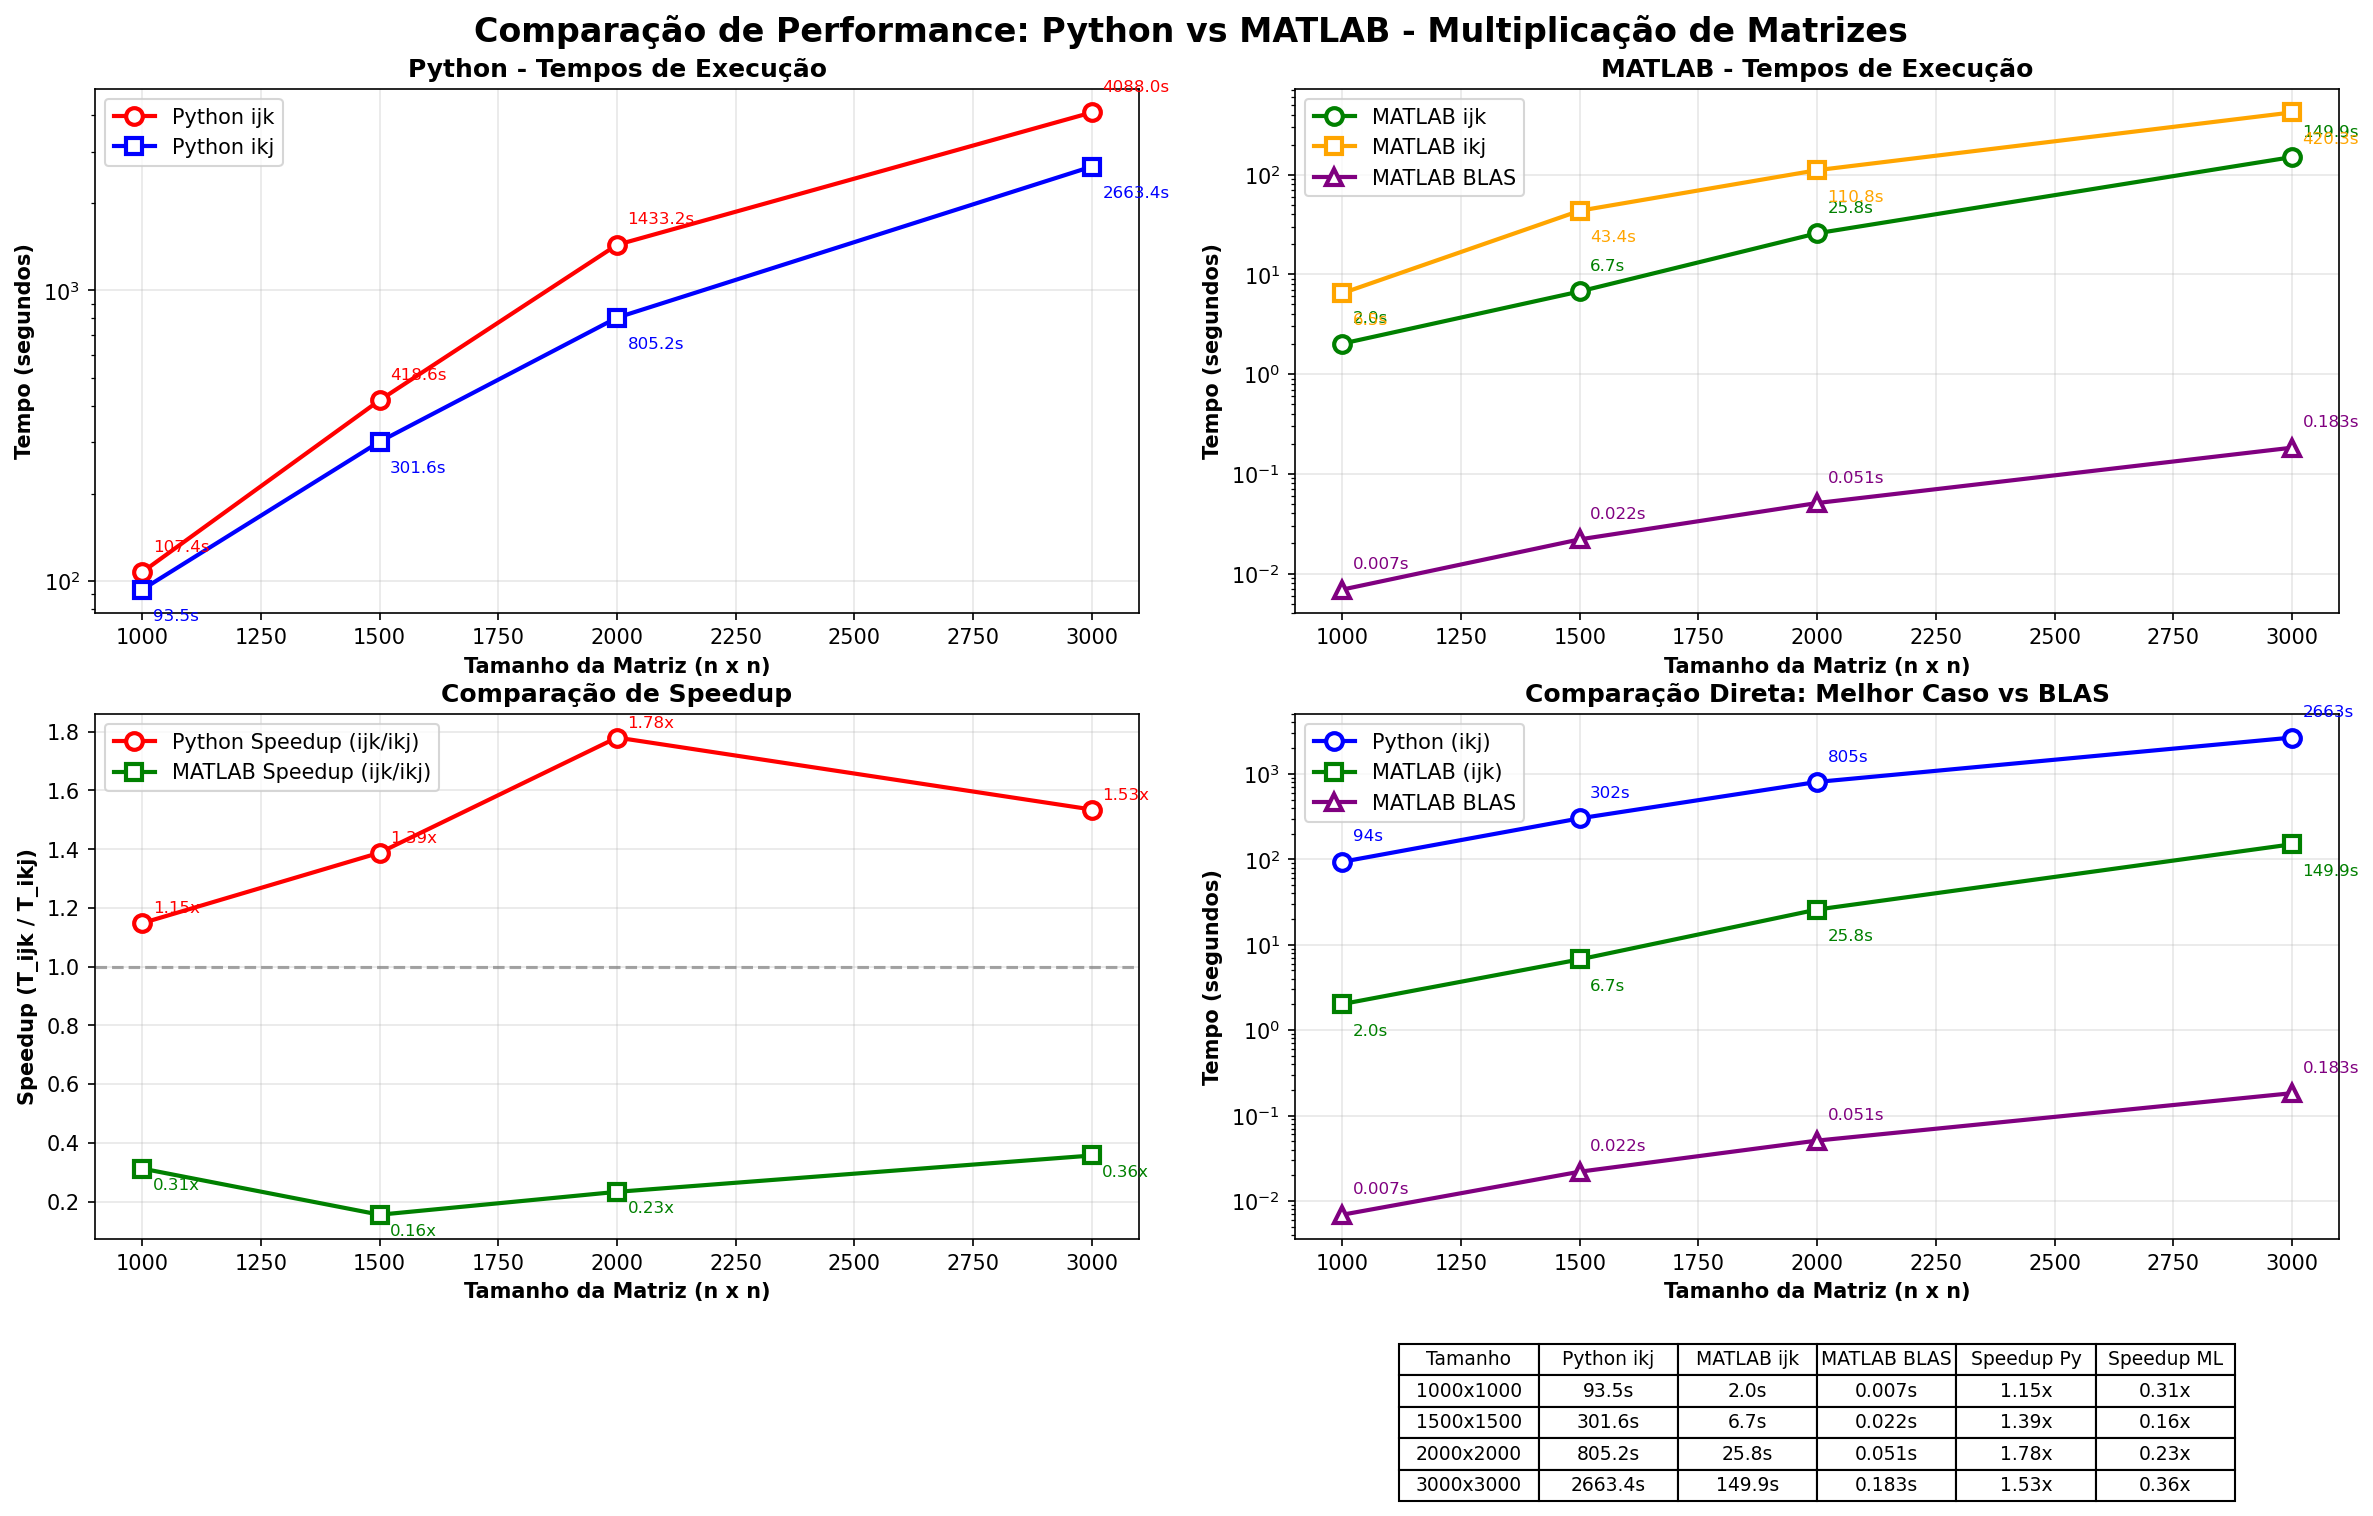
\includegraphics[width=0.80\linewidth]{Figuras/comparacao_python_matlab}
		\caption{Python vs Matlab}
		\label{fig:performace_python_vs_matlab}
	\end{figure}
\end{frame}

\end{document}
